\documentclass[a4,fleqn]{article}
\usepackage{amsmath, amsthm}
\usepackage{mathtools}
%\usepackage{color}
%\usepackage{svgcolor}
\usepackage{amsfonts}
\usepackage{tikz}
\usetikzlibrary{arrows,snakes,backgrounds}

%new_commands.tex

\newcommand{\R}{\mathbb{R}}

\newcommand{\MWT}{Minkowski-Weyl Theorem}
\newcommand{\FME}{Fourier-Motzkin Elimination}
\newcommand{\MSum}{Minkowski Sum}
\newcommand{\suchthat}{\;|\;}
\renewcommand{\vec}[1]{\mathbf{#1}}
\newcommand{\x}{\vec{x}}
\newcommand{\e}{\vec{e}}
\renewcommand{\b}{\vec{b}}
\newcommand{\w}{\vec{w}}
\newcommand{\z}{\vec{z}}
\renewcommand{\a}{\vec{a}}
\newcommand{\stack}[2]{\begin{pmatrix}#1 \\ #2\end{pmatrix}}
\newcommand{\smallstack}[2]{\left(\begin{smallmatrix}#1 \\ #2\end{smallmatrix}\right)}
\newcommand{\xx}{\stack{x_0}{\x}}

\newcommand{\dotproduct}[2]{\langle #1, #2 \rangle}
\newcommand{\convComb}[3]{#3 #1 + (1-#3) #2}
\newcommand{\convCombb}[3]{\sum\nolimits_{#3} #2_{#3} #1_{#3}}

\newcommand{\Hedron}[2]{\mathcal{#1}_{\mathcal{#2}}}
\newcommand{\PV}{\Hedron{P}{V}}
\newcommand{\CV}{\Hedron{C}{V}}
\newcommand{\PH}{\Hedron{P}{H}}
\newcommand{\CH}{\Hedron{C}{H}}
\newcommand{\CVp}{\Hedron{C}{V'}}
\newcommand{\CHp}{\Hedron{C}{H'}}
\newcommand{\F}{\mathcal{F}}

\newcommand{\todo}[1]{\textcolor{red}{(#1)}}

\DeclareMathOperator{\conv}{conv}
\DeclareMathOperator{\cone}{cone}


\newtheorem{thm}{Theorem}
\newtheorem{lemma}{Lemma}
\newtheorem{claim}{Claim}
\newtheorem{definition}{Definition}
\begin{document}
\textcolor{blue}{The input is blocked from what I've done so far, I will attempt to do a rewrite of part of the proof to make sure I have the right ``style''}

\newcommand{\bset}[1]{\left\{#1\right\}}
\newcommand{\hcone}[1]{\bset{\x \in \R^d \suchthat #1\x \leq \vec{0}}}
\newcommand{\vcone}[1]{\bset{\x \in \R^d \suchthat 
                            \exists \t \in\R^n\geq \vec{0},\, \x = #1\t}}
\newcommand{\mdef}[3]{#1 \in \R^{#2 \times #3}}
\newcommand{\hplane}[2]{\bset{\x \in \R^{#1} \suchthat x_{#2} = 0}}
\newcommand{\svec}[2]{\begin{pmatrix*}[c] #1 \\ #2 \end{pmatrix*}}

\newcommand{\uvsum}{\sum_{\substack{ i \in P \\ j \in N }}}

\subsection{Notation}  
The canonical basis vectors will be written $\e_k$ for valid values of $k$.  Let $\x \in \R^n$.  It will be customary to write:
  \[x_k = \dotproduct{\e_k}{\x}\]
Given $\mdef{A}{m}{d}$, Let $A_i$ and $A^j$ denote the rows and columns of $A$, respectively.  Then $A^j_i$ will denote the entry from $A$ in the $i$-th row and $j$-th column.  Matrix multiplication is then given by:
\[ A\x = \sum_{j=1}^{d} A^j x_j = 
  \begin{pmatrix} 
    \dotproduct{A_1}{\x} \\ \vdots \\ \dotproduct{A_m}{\x}
  \end{pmatrix} =
  \sum_{i=1}^m \dotproduct{A_i}{\x} \e_i
\]
Let $\x \in \R^d$, $\w \in \R^m$, and define the following notation for vectors in $\R^{d+m}$:
\begin{align*}
  \dotproduct{\e_k}{\svec{\x}{\w}} = 
    \begin{cases} x_k     & k \leq d \\
                  w_{k-d} & d+1 \leq k \leq d+m
    \end{cases}
\end{align*}

\hrule \bigskip

\subsection {Definitions}

\begin{definition}[H-Cone]{
  Let $\mdef{A}{m}{d}$, then define 
  \[\CH(A) = \hcone{A}\]
} \end{definition}

\begin{definition}[V-Cone]{
  Let $\mdef{V}{d}{n}$, then define 
  \[\CV(V) = \vcone{V}\]
  A vector of the form $V\t$, where $\t \geq \vec{0}$ is called a ``conical combination of V''.
} \end{definition}

\begin{definition}[Hyperplane]{
  Let $\a \in \R^n, b \in \R$.  Then the set
  \[ \{\x \in \R^n \suchthat \dotproduct{\a}{\x} = b\} \]
  Is known as a hyperplane.  Let $H_{k}^{n} \subseteq \R^n$ denote the hyperplane defined by:
  \[H_{k}^{n} = \hplane{n}{k}\]
} \end{definition}

\begin{definition}[Projection]{
  Let $\x\in\R^d$.  The vector $\x'\in\R^{d-k}$ formed by omitting $k$ coordinates of $\x$ is called a projection of $\x$.  In particular, let $\x\in\R^d, \w\in\R^m$, and $\smallstack{\x}{\w} \in \R^{d+m}$, and define ${\pi_{\x} : \R^{d+m} \to \R^{d}}$ as:
  \[ \pi_{\x} \svec{\x}{\w} = \x \]
  Then $\pi_{\x}$ is a projection onto the first d-coordinates.
} \end{definition}

\paragraph{Remarks:}  In the following sections it will be proved that every \textbf{H-Cone} is a \textbf{V-Cone}, and every \textbf{V-Cone} is an \textbf{H-Cone}.  This shows that these are two fundamentally different descriptions of the same object.  Each has its own power and purpose, which will be discussed later.

Let $A \subseteq \R^n$.  Then $A \cap H_k^n$ is simply all of the points of $A$ who have the $k$-th coordinate $0$.  Let $\pi^k$ be the projection that omits the $k$-th coordinate.  Then $\pi^k(A \cap H_k^n)$ are all the points of $A$ whose $k$-th coordinate is $0$, but without that $0$ coordinate.  If projections are thought of as ``forgetting useless information,'' and intersections as ``capturing only the useful information,'' then the sequence of projection and intersection is ``capturing the useful information, and forgetting the useless information.''

\subsection {H-Cone $\to$ V-Cone}

\begin{thm}{\label{thm:htov}
  Let $\mdef{A}{m}{d}$, then for the set $\CH(A)$, there exists a ${\mdef{V}{d}{n}}$ such that 
  \[\CH(A) = \CV(V)\]
} \end{thm}
\hrule
\begin{claim}{\label{claim:htovlift}
  Let $\mdef{A}{m}{d}$.  Then there exists a $\mdef{V'}{(d+m)}{(2d+m)}$ such that 
  \[\CH(A) =  \left\{ \x \in \R^d \Suchthat 
              \svec{\x}{\vec{0}} \in \CV(V') \right\}
  \]
} \end{claim}

\begin{claim}{\label{claim:htovproject}
  \[  \left\{ \x \in \R^d \Suchthat 
              \svec{\x}{\vec{0}} \in \CV(V') \right\}
           = \pi_{\x} \left(\CV(V') \bigcap_{k=d+1}^{d+m} H_k^{d+m}\right)\]
} \end{claim}

\begin{claim}{\label{claim:htovdrop}
  Let $\mdef{V'_{in}}{(d+m)}{n_{in}}$, then there exists a set $\mdef{V'_{out}}{(d+m)}{n_{out}}$ such that
 \[ \CV(V'_{in}) \cap H_{k}^{d+m} = \CV(V'_{out}) \]
\paragraph{Note:} $V'_{in}$ and $V'_{out}$ are intended to represent ``input'' and ``output'' sets - this claim is true by the existence of an algorithm shown later.
} \end{claim}

\begin{claim}{\label{claim:htovcvproject}
  Let $\mdef{V'}{(d+m)}{n}$, then 
 \[ \pi_{\x}(\CV(V') = \CV(\pi_{\x}(V')) \]
} \end{claim}

\bigskip \hrule

\begin{proof}[Proof of \textnormal{\textbf{Theorem \ref{thm:htov}}}]
Theorem \ref{thm:htov} follows from the claims as follows.  First, apply claim \ref{claim:htovlift} to $A$ to get a set $V'$ of vectors in $\R^{d+m}$.  Claim \ref{claim:htovproject} shows us that the set $\CH(A)$ can be formed by first taking a finite number of intersections of $\CV(V')$ with hyperplanes of the form $H_k^{d+m}$, then projecting this set onto $\x$.  Claim \ref{claim:htovdrop} gives us a method to eliminate all of the intersections in the form given by claim \ref{claim:htovproject}, and end up with a set $V''$ with the following useful property:
\[  \CV(V'') \bigcap_{k=d+1}^{d+m} H_k^{d+m} = \CV(V'') \]
Claim \ref{claim:htovcvproject}, along with the set $V''$, allows the following calculation:
\[ \CH(A) = \pi_{\x} \left(\CV(V'') \bigcap_{k=d+1}^{d+m} H_k^{d+m}\right)
          = \pi_{\x} (\CV(V'')) = \CV(\pi_{\x}(V''))
\]
Letting $V = \pi_{\x}(V'')$, we then have 
\[ \CH(A) = \CV(V) \]
\end{proof}
\paragraph{Remarks:}  Discussing ``what is hard'' is helpful for understanding the proof and why it is formed the way it is.  Claim \ref{claim:htovlift} is not terribly difficult, it mostly just takes a clever idea and attention to detail.  It is reminiscent of techniques common to linear programming.  Claims \ref{claim:htovproject} and \ref{claim:htovcvproject} are very straightforward, they exist primarily to make the proofs of the other claims less cluttered.  Claim \ref{claim:htovdrop} is really the ``main'' idea that needs proving.  This is because intersecting a V-Cone with a set of the form $H_k^{d+m}$ requires determining all vectors of the V-Cone $\CV(V')$ that have a $0$ in the $k$-th coordinate.  Only conical combinations of $V'$ of a special form will have this property, determining this form is the heart of the proof.  Using the language from the above remark, ``forgetting the useless information is easy, capturing the important information is hard, and representing the information in a different way is tricky.''

\bigskip \hrule
\bigskip
\textbf{Claim \ref{claim:htovlift}:} \textit{ Let $\mdef{A}{m}{d}$.  Then there exists a $\mdef{V'}{(d+m)}{(2d+m)}$ such that}
  \[\CH(A) =  \left\{ \x \in \R^d \Suchthat 
              \svec{\x}{\vec{0}} \in \CV(V') \right\}
  \]

\begin{proof}[Proof of \textnormal{\textbf{Claim \ref{claim:htovlift}}}(tricky)]
Define $V'$:
\[ V' = \bset{\pm\svec{\e_j}{A^j}, \svec{\vec{0}}{\e_i} \Suchthat 1\leq j \leq d, 1 \leq i \leq m} \]
Let $\x \in \CH(A)$.  Then it is to be shown that:
\[ A\x \leq \vec{0} \Rightarrow \svec{\x}{\vec{0}} \in \CV(V') \]
The task is to find a $t_j^+,t_j^-,w_i \geq 0$ such that:
 \[ \svec{\x}{\vec{0}} = \sum_{j=1}^{d} t_j^+ \svec{\e_j}{A^j} -
                        \sum_{j=1}^{d} t_j^- \svec{\e_j}{A^j} +
                        \sum_{i=1}^{m} w_i \svec{\vec{0}}{\e_j} \]
Consider the following assignments:
\begin{align*}
  t_j^+ &= \begin{cases} x_j & x_j \geq 0 \\ 0   & x_j < 0 \end{cases} \\
  t_j^- &= \begin{cases} 0   & x_j \geq 0 \\ -x_j & x_j < 0 \end{cases} \\
  w_i   &= -\dotproduct{A_i}{\x}
\end{align*}
By the way we've defined $t_j^+$ and $t_j^-$, $x_j = t_j^+ - t_j^-$.  Then:
\begin{align*} \sum_{j=1}^{d} t_j^+ \svec{\e_j}{A^j} -
                 \sum_{j=1}^{d} t_j^- \svec{\e_j}{A^j} =
               \sum_{j=1}^{d} (t_j^+ - t_j^-) \svec{\e_j}{A^j} = 
               \sum_{j=1}^{d} x_j \svec{\e_j}{A^j} =
               \svec{\x}{A\x}
\end{align*}
Furthermore:
\[ \sum_{i=1}^{m} w_i \svec{\vec{0}}{\e_i} 
      = -\sum_{i=1}^{m} \dotproduct{A_i}{\x} \svec{\vec{0}}{\e_i} 
      = \svec{\vec{0}}{-A\x} \]
It is clear that $t_j^+,t_j^- \geq 0$, and $w_i \geq 0$ follows from $A\x \leq \vec{0}$.  It follows that:
\begin{align*} &\sum_{j=1}^{d} t_j^+ \svec{\e_j}{A^j} -
                 \sum_{j=1}^{d} t_j^- \svec{\e_j}{A^j} +
                 \sum_{i=1}^{m} w_i \svec{\vec{0}}{\e_i} \in \CV(V')
\end{align*}
Combining results, we have:
 \[ \sum_{j=1}^{d} t_j^+ \svec{\e_j}{A^j} -
      \sum_{j=1}^{d} t_j^- \svec{\e_j}{A^j} +
      \sum_{i=1}^{m} w_i \svec{\vec{0}}{\e_j} =
    \svec{\x}{A\x} + \svec{\vec{0}}{-A\x}  = \svec{\x}{\vec{0}} \]
And we conclude that $\svec{\x}{\vec{0}} \in \CV(V')$.

Now let $\svec{\x}{\vec{0}} \in \CV(V')$.  The task is to show that $A\x \leq 0$.  We have:
\begin{align*} 
   \svec{\x}{\vec{0}} = &\sum_{j=1}^{d} t_j^+ \svec{\e_j}{A^j} -
                        \sum_{j=1}^{d} t_j^- \svec{\e_j}{A^j} +
                        \sum_{i=1}^{m} w_i \svec{\vec{0}}{\e_j} =&\Suchthat
                        t_j^+,t_j^-,w_i \geq 0 \\
                        &\sum_{j=1}^{d} (t_j^+-t_j^-) \svec{\e_j}{A^j} +
                        \sum_{i=1}^{m} w_i \svec{\vec{0}}{\e_j} &\Suchthat
                        t_j^+,t_j^-,w_i \geq 0
\end{align*} 
Since the only contribution to the coordinate of $x_j$ is $t_j^+ - t_j^-$, we may conclude that $x_j = t_j^+ - t_j^-$.  Continuing the string of equalities:
\begin{align*} 
                        &\sum_{j=1}^{d} (t_j^+-t_j^-) \svec{\e_j}{A^j} +
                        \sum_{i=1}^{m} w_i \svec{\vec{0}}{\e_j} =&\Suchthat
                        t_j^+,t_j^-,w_i \geq 0 \\
                        &\sum_{j=1}^{d} x_j \svec{\e_j}{A^j} +
                        \sum_{i=1}^{m} w_i \svec{\vec{0}}{\e_j} =&\Suchthat
                        w_i \geq 0, x_j \in \R \\
                        &\svec{\x}{A\x} + \svec{\vec{0}}{\w} = 
                            \svec{\x}{\vec{0}}
                                                                 &\Suchthat
                        \w \geq \vec{0}, \x \in \R^d
\end{align*} 
This last line implies that $A\x + \w = \vec{0} \Rightarrow A\x = -\w \leq \vec{0}$.
\end{proof}
\bigskip \hrule \bigskip

\textbf{Claim \ref{claim:htovproject}:}
  \[  \left\{ \x \in \R^d \Suchthat 
              \svec{\x}{\vec{0}} \in \CV(V') \right\}
           = \pi_{\x} \left(\CV(V') \bigcap_{k=d+1}^{d+m} H_k^{d+m}\right)\]
\begin{proof}[Proof of \textnormal{\textbf{Claim \ref{claim:htovproject}}}(easy)]
\begin{align*}
  \CV(V') \bigcap_{k=d+1}^{d+m} H_k^{d+m}
    &= \left\{ \z \in \CV(V') \Suchthat z_k = 0 : d+1 \leq k \leq d+m \right\} \\
    &= \left\{ \svec{\x}{\w} \in \CV(V') \Suchthat 
          \x \in \R^d, \w \in \R^m, w_k = 0 : 1 \leq k \leq m \right\} \\
    &= \left\{ \svec{\x}{\w} \in \CV(V') \Suchthat 
          \x \in \R^d, \w \in \R^m, \w = \vec{0} \right\} \\
    &= \left\{ \svec{\x}{\vec{0}} \in \CV(V') \Suchthat \x \in \R^d \right\}
\end{align*}
Then
  \[ \pi_{\x}\left(\CV(V') \bigcap_{k=d+1}^{d+m} H_k^{d+m}\right) 
      = \left\{ \x \in \R^d \Suchthat \svec{\x}{\vec{0}} \in \CV(V') \right\} \]
      
\end{proof}

\bigskip \hrule \bigskip

The following lemma will be useful in the upcoming proof.
\begin{lemma}[Subcone]{\label{lemma:subcone}
  $U \subseteq \CV(V) \Rightarrow \CV(U) \subseteq \CV(V)$
} \end{lemma}
\begin{proof}
For any $\u^i \in U$ we have $\u^i = \sum_j t_{ij} \v^j$.  Then, for any conical combination of $\u^i$ we have:
\[ \sum\nolimits_i s_i\u^i 
        = \sum\nolimits_i s_i\left(\sum\nolimits_j t_{ij} \v^j\right)
        = \sum\nolimits_j \left(\sum\nolimits_i s_i t_{ij}\right) \v^j
\]
Since $s_i, t_{ij} \geq 0$, the final expression is a conical combination of $V$.
\end{proof}

\bigskip \hrule \bigskip

\textbf{Claim \ref{claim:htovdrop}:} \textit{Let $\mdef{V'_{in}}{(d+m)}{n_{in}}$, then there exists a set $\mdef{V'_{out}}{(d+m)}{n_{out}}$ such that}
 \[ \CV(V'_{in}) \cap H_{k}^{d+m} = \CV(V'_{out}) \]
\begin{proof}[Proof of \textnormal{\textbf{Claim \ref{claim:htovdrop}}}(hard)]
Suppose that the vectors of $V_{in}$ are indexed by a set $I$.  We partition the vectors of $V_{in}$ based on their value at coordinate $k$.
\begin{align*}
  P = i \in I &\suchthat v_k^i > 0 \\
  N = j \in I &\suchthat v_k^j < 0 \\
  Z = l \in I &\suchthat v_k^l = 0
\end{align*}
Here, we've used different indices $i,j,l$.  This is purely for convenience, and in what follows we'll follow the convention that $i\in P$, $j \in N$, and $l \in Z$.
Next, let
\[ V_{out} = \{ \v^l \suchthat l \in Z\} \cup 
      \{v^i_k \v^j - v^j_k \v^i \suchthat i \in P, j \in N \} \]
There are two critical properties of the set $V_{out}$. First, every $\v \in V_{out}$ is formed by taking conical combinations of vectors from $V_{in}$.  Also, for any $\v \in V_{out}$, we have that $v_k = 0$.  These two properties, along with lemma \ref{lemma:subcone} gives 
\[ \CV(V_{out}) \subseteq \CV(V_{in}) \cap H^{d+m}_k \]

Next, say $\x \in \CV(V_{in}) \cap H^{d+m}_k$, then:
\begin{align*}
\x &= \sum_{i \in P}t_i\v^i + \sum_{j \in N} t_j\v^j + \sum_{l \in Z} t_l\v^l
\end{align*}
Because $x_k = 0$, and $v^l_k = 0$ for each $l \in Z$, we have
\begin{align*}
 0 &= \sum_{i \in P}t_i v^i_k + \sum_{j \in N} t_j v^j_k + \sum_{l \in Z} t_l v^l_k \\
   &= \sum_{i \in P}t_i v^i_k + \sum_{j \in N} t_j v^j_k
\end{align*}
This final line implies that the sums have opposite values.  Denote this value by $\tau$, that is
\[ \tau = \sum_{i \in P}t_i v^i_k = -\sum_{j \in N} t_j v^j_k \]
If $\tau = 0$, then each $t_i,t_j = 0$ and $\x$ is a conical combination of vectors from $\v^l : l \in Z$, and therefore $\x \in \CV(V_{out})$.  Suppose that $\tau > 0$.  Then we have
\begin{align*} 
 &\sum_{i \in P}t_i \v^i 
   = \frac{-1}{\tau}\sum_{j \in N}t_j v^j_k \sum_{i \in P}t_i \v^i 
   = -\uvsum \frac{t_i t_j}{\tau} v^j_k \v^i \\[1em]
 &\sum_{j \in N}t_j \v^j 
   = \,\frac{1}{\tau}\sum_{i \in N}t_i v^i_k \sum_{j \in P}t_j \v^j 
   = \quad\uvsum \frac{t_i t_j}{\tau} v^i_k \v^j
\end{align*}
Combining these results, we have:
\begin{align*}
   \sum_{i \in P}t_i \v^i + \sum_{j \in N}t_j \v^j 
   &= \uvsum \frac{t_i t_j}{\tau} v^i_k \v^j 
      - \uvsum \frac{t_i t_j}{\tau} v^j_k \v^i \\
   &=  \uvsum \frac{t_i t_j}{\tau}(v^i_k\v^j - v^j_k\v^i)
\end{align*}
Because $\tau > 0, t_i,t_j \geq 0$, it follows that $\frac{t_i t_j}{\tau} \geq 0$.  This shows that the sum above can be written as a conical combination of vectors from $V_{out}$.  We can now rewrite $\x$:
\begin{align*}
\x &= \sum_{i\in P}t_i\v^i + \sum_{j\in N} t_j\v^j + \sum_{l\in Z} t_l\v^l \\
   &=  \uvsum \frac{t_i t_j}{\tau}(v^i_k\v^j - v^j_k\v^i) +
        \sum_{l \in Z} t_l \v^l
\end{align*}
This shows $\x$ is a conical combination of vectors from $V_{out}$, so 
\[ \CV(V_{in}) \cap H^{d+m}_k \subseteq \CV(V_{out}) \]
\end{proof}

\bigskip \hrule \bigskip

\textbf{Claim \ref{claim:htovcvproject}:}
  \textit{Let $\mdef{V'}{(d+m)}{n}$, then }
 \[ \pi_{\x}(\CV(V') = \CV(\pi_{\x}(V')) \]
\begin{proof}[Proof of \textnormal{\textbf{Claim \ref{claim:htovcvproject}}}(easy)]
This follows from the fact that projections are linear transformations.  Take the projection:
\[ \pi_{\x}\svec{\x}{\w} = \x\]
Then
\[ \pi_{\x}\left( \alpha \svec{\x}{\w} + \svec{\y}{\z}\right) = 
    \pi_{\x}\svec{\alpha \x + \y}{\alpha \w + \z} = \alpha \x + \y =
    \alpha \pi_{\x}\svec{\x}{\w} + \pi_{\x}\svec{\y}{\z} \]
Let $J$ index the vectors of $V'$.  Say $\v \in \CV(V')$, then
\[ \pi_{\x}(\v) = \pi_{\x}\left(\sum_{j\in J}t_j\v^j\right) = 
      \sum_{j\in J}t_j\pi_{\x}(\v^j) \]
This is apparently a conical combination of vectors from $\pi_{\x}(V')$, so $\v \in \CV(\pi_{\x}(V'))$.

Similarly, say $\u \in \CV(\pi_{\x}(V'))$, then
\[ \u = \sum_{j\in J}t_j\pi_{\x}(\v^j) = 
      \pi_{\x}\left(\sum_{j\in J}t_j\v^j\right)\]
So $\u \in \pi_{\x}(\CV(V'))$.
\end{proof}

%
%\section{Introduction}
%%introduction.tex

% importance
The \MWT{} is a theorem of utmost importance in the theory of polyhedra.  Ziegler refers to it as the ``main theorem.''  It is a theorem which is easy to intuitively understand, but is surprisingly difficult to prove.  Going through the proof in detail, however, is a good excersice because it introduces various other imporant notions and techniques, as well as helps to mentally clarify the basic definitions relevant to the theory.

Polyhedra are ``finitely generated'' convex subsets of $\R^n$.  ``Finitely generated'' here means that they can be described in a finite manner, in particular as a convex hull of either: a finite set of points and ray, or a finite intersection of halfspaces.  The \MWT{} states that these two finite representations are ``equivalent,'' that every polyhedra can be described either way.

For a more concrete example, consider a polygon in the plane \todo{provide some nice pictures here}.

% paper overview
In this paper, the theorem and relvant definitions will be stated, and a proof will be given.  The proof will closely follow Ziegler's, however it is the author's intent to make this paper as accessible as possible \todo{who is the target audience?}.  Therefore, some concepts will be stated in somewhat more painstaking detail than some may find necessary, however these details will have to be addressed to implement an enumeration-algorithm that will accompany the proof.

% diagram
Perhaps the most important part of the paper is the diagram in figure \ref{fig:proof}.  This diagram illustrates the main steps of the proof, and will serve as a ``roadmap'' to the implementation.


%
%\section{Definitions}
%
\subsection{Informal Notions}
% informal notions

Here shall be stated some of the fundamental ideas involved in the theory of polyhedra (formal definitions will be given in the next section).

\paragraph{Convexity} Convexity is an essential notion in the study of polyhedra.  Here, it will be considered a property of subsets of $\R^n$.  Let $A \subseteq \R^n$.  A is \textit{convex} if, given any two points of $A$, the line segment connecting these two points is also contained in $A$.  It formalizes a notion of being ``filled-in,'' and implies that (given the standard metric) the shortest path between any two points of $A$ is included in $A$.  

\paragraph{Convex Hulls} Associated with the notion of convexity is the operation of \textit{convex hull}.  Given any subset $B \subseteq \R^n$, the \textit{convex hull} of $B$ is the smallest set which contains $B$ and is convex.  For two isolated points, their convex hull is the line segment with the given points as endpoints.  For more complex sets, it can be thought of as in iterative procedure where the convex hull of every two points is added to the set, repeating this operation until no more points are added. \todo{a picture showing how the procedure must iterate}.

\paragraph{Minkowski Sums}

%- Important transforms
\paragraph{Projections, Lifts, Relaxations, Restrictions}  These terms will be will be used informally in this paper, however when one is needed in a formal context it will be specified as necessary.  

\textit{Projections} are very simple operations, which basically cause one to ``ignore'' the coordinates of a set for a given index set of coordinates.  For example, $\pi: (x,y) \mapsto (x)$ is a projection from $\R^2$ to $\R$.  Projections are often given a subscript to indicate which dimensions are being ``projected to,'' or a superscript to indicate which dimensions are being ``projected away.''  So $\pi$ above may be written as $\pi_x$ or perhaps $\pi^y$, however in formal contexts the precise nature of the projection will be indicated; this notation is meant only to be useful for the reader.

A \textit{lift} refers to taking a set and representing it in a higher dimension.  For example, one may take the unit interval $I = [0,1] \subseteq \R^1$ and \textit{lift} it to $\R^2$ by considering $I \times {0}$.  

\textit{Relaxations and Restrictions}: A \textit{relaxation} of a set will typically be a way to let a set ``grow,'' however it will typically be in a ``controlled'' or ``reversible'' manner.  These ``reversals'' will be referred to as \textit{restrictions}.  Take, for instance, this relaxation of the unit interval $I = [0,1]$: 
  \[\bigcup_{t \geq 0} [0,t]\times t \quad=\quad 
    \{(x,y) \suchthat x \geq 0\} \cap \{(x,y) \suchthat y - x \geq 0\}\]  
From this relaxation (an ``infinite triangle'' of sorts) we may recover $I$ with a respective restriction, in this case by intersecting the relaxation with ${\{(x,y) \suchthat y = 1\}}$ and projecting it to the x axis.  Again, the terms \textit{relaxation} and \textit{restriction} will be used informally, while specific instances will be specified as needed.


\subsection{Formal Definitions}
Here are the formal defintions required for the statement of the theorem and its proof.  In all definitions, unless otherwise stated, $I$ represents and arbitray \textit{finite} index set, and $J$ is an \textit{arbitrary} index set.

% convex combination
\paragraph{Convex Combination} 
Let $\vec{x},\vec{y} \in \R^n,\, \lambda \in [0,1]$.  Then
  \[\convComb{\vec{x}}{\vec{y}}{\lambda}\]
is called a \textit{convex combination} of $\vec{x}$ and $\vec{y}$.
More generally, $\vec{x}_i \in \R^n$, $\lambda_i \in [0,1]$, and $\sum_i \lambda_i = 1$.  Then 
  \[\convCombb{\vec{x}}{\lambda}{i}\]
is called a \textit{convex combination} of $\vec{x}_i$.

% convex
\paragraph{Convex} 
Let $A \subseteq R^n$.  $A$ is by definition \textit{convex} if every convex combination of its members is again a member.  In symbols:
  \[\vec{x}_i \in A \Rightarrow
    \convCombb{\vec{x}}{\lambda}{i} \in A\]
Note: Let $(\forall j \in J) \, A_j \subseteq \R^n$ be convex, and $(\forall i\in I)\,\vec{x}_i, \in \bigcap_{j\in J}A_j$.  Then 
  \[(\forall j\in J)\; \convCombb{\vec{x}}{\lambda}{i} \in A_j \Rightarrow \convCombb{\vec{x}}{\lambda}{i} \in \bigcap_{j \in J} A_j\]  
 This implies that $\bigcap_{i \in I} A_i$ is also convex.  In other words, the property of being convex is closed under the operation of intersection.

% halfspace
\paragraph{Halfspace}
Let $\vec{y} \in \R^n,\, c \in \R$.  Then the set
  \[ \{\vec{x} \suchthat \dotproduct{\vec{x}}{\vec{y}} \leq c\} \]
is called a \textit{halfspace}.  In particular, $H_k$ shall denote the halfspace given by
  \[ \{\vec{x} \suchthat \dotproduct{\vec{x}}{\vec{e}_k} \leq 0 \} = 
     \{\vec{x} \suchthat x_k \leq 0 \} \]
Note:  Suppose that 
  $\dotproduct{\vec{x}}{\vec{y}} \leq c,\;$ 
  $\dotproduct{\vec{z}}{\vec{y}} \leq c,\;$ and
  $\lambda \in [0,1]$.  Then
  \[ \dotproduct{\convComb{\vec{x}}{\vec{z}}{\lambda}}{\vec{y}} = 
    \convComb{\dotproduct{\vec{x}}{\vec{y}}}
             {\dotproduct{\vec{z}}{\vec{y}}}
             {\lambda} \leq \convComb{\cdot c}{\cdot c}{\lambda} = c
  \]
  This means that halfspaces are \textit{convex}.

% H-polyhedron
\paragraph{H-polyhedron}
An \textit{H-polyhedron} is a finite intersection of halfspaces.  By the remark given under the definition of \textbf{convexity}, \textit{H-polyhedra are convex.}  Here is a useful way of ``writing down'' an H-polyhedron:
  \[ \{ \vec{x} \in \R^n \suchthat 
    \forall i:\, \dotproduct{\vec{x}}{\vec{a}_i} \leq b_i \} \]
If all the $\vec{a}_i$ are gathered into a matrix $A$ (where the $\vec{a}_i$ become the rows of $A$), this is sometimes also written as:
  \[ \{ \vec{x} \in \R^n \suchthat A\vec{x} \leq \vec{b} \} \]

% -convex-hull
\paragraph{Convex Hull}
Let $A \subseteq \R^n$.  $B$ is by definition the \textit{convex-hull} of $A$ if
  \[ B = \conv(A) = \{ \vec{x} \suchthat \exists \vec{a}_i \in A, \exists\lambda_i \in [0,1]: \sum_i \lambda_i = 1,\,\vec{x} = \convCombb{\vec{a}}{\lambda}{i} \} \]

Note: Another useful, equivalent definition of \textit{convex hull} can be given as:
\[ B' = \conv'(A) = \bigcap \{C \suchthat 
      A \subseteq C, \, C \text{ is convex}\} \]
This more clearly illustrates the idea of ``smallest convex set containing $A$.''  To see that these definitions are equivalent, first note that $B$ is convex, and $A \subseteq B$, so $B' \subseteq B$ (since $B$ will be included in the intersection).  Then note that if $C$ is convex and $A \subseteq C$, then any convex combination of members of $A$ must (by definition) be in $C$, so it will be in every such $C$ and therefore in their intersection, so $B' \subseteq B.$

% conical hull
\paragraph{Conical Hull}  Let $\cup_{i\in I} \vec{a}_i = A \subseteq \R^n$, then $B$ is by definition the \textit{conical hull} of $A$ if:
  \[ B = \cone(A) = \{ \vec{x}\in \R^n \suchthat\; \exists t_i \in \R^n \suchthat \; t_i \geq 0,\; \vec{x} = \sum_{i\in I} t_i\vec{a}_i \} \]

Note: A conical hull is convex.  Let $K,\, (\forall i\in I)\, J_i$ be finite index sets (i.e. $J_i$ is a collection of finite index sets, indexed by the finite set $I$), $(\forall i \in I)(j \in J_i): t_{i,j} \geq 0,\, \vec{a}_{i,j} \in A$, and, as usual, $\lambda_i \in [0,1],\, \sum_i \lambda_i = 1$.  Then
  \[ \sum\nolimits_i \lambda_i \left(\sum\nolimits_{j \in J_i} t_{i,j} \vec{a}_{i,j}\right) = \sum\nolimits_{i,j\in J_i} \lambda_i \cdot t_{i,j} \vec{a}_{i,j}\]
is a ``conical combination'' of vectors in $A$ (because $\lambda_i\cdot t_{i,j} \geq 0$), so every convex combination from $\cone(A)$ is again in $\cone(A)$.

% minkowski sum
\paragraph{Minkowski Sum}
Let $P,Q \subseteq \R^n$.  Then the \textit{Minkowski Sum} of $P$ and $Q$ is given by:
  \[ P \oplus Q = \{ p + q \suchthat p \in P,\, q \in Q \} \]

Note:  If both $P$ and $Q$ are convex, then so is $P \oplus Q$.  Indeed, let $p_i \in P,\, q_i \in Q$, then
  \[\sum_i\nolimits \lambda_i(p_i + q_i) = 
  \convCombb{p}{\lambda}{i} + \convCombb{q}{\lambda}{i} = 
  \bar{p} + \bar{q}
  \]
Where $\bar{p} \in P$ and $\bar{q} \in Q$ (because they are convex), so $\bar{p} + \bar{q} \in P \oplus Q$.

% V-polyhedron
\paragraph{V-Polyhedron}  A \textit{V-Polyhedron} is a subset $\mathcal{P}$ of $\R^n$ given by 
  \[ \mathcal{P} = \cone(\mathcal{U}) \oplus \conv(\mathcal{V}) \] 
where $\mathcal{U}$ and $\mathcal{V}$ are both finite (possibly empty) subsets of $\R^n$.  By the remark given under the definition of Minkowski Sums, \textit{V-Polyhedra are convex}.

\bigskip
\noindent We are now prepared to state the \MWT.

% statement of theorem
\paragraph{\MWT}
Every V-Polyhedron is an H-Polyhedron, and every H-Polyhedron is a V-Polyhedron.  This permits the use of the term ``Polyhedron'' unambiguously.
\medskip

Note:  I've read that ``definitions should be hard and theorems should be easy.''  Perhaps there is a bit of this involved in the \MWT{}, but an unfortunate side effect is that the significance of a theorem may not be immediate.  The \MWT{} is a ``representation theorem,'' and is a consequence of a type of duality that exists between the V and H --type definitions of polyhedra.

For a quick demonstration of why a dual representation is important for these types of sets, consider the following two tasks:
\begin{itemize}
  \item Given a point $\vec{x}$, determine if it is a member of the set
  \item Produce an arbitrary member of the set
\end{itemize}
These two fundamental tasks tell completely different stories given one representation as opposed to the other.  For an H-Polyhedron, determining membership is straightforward and relatively inexpensive: for each halfspace constraint, check to see that it is fulfilled.  For a V-Polyhedron, you would need to either find a combination that produces the point, or provide a ``certificate'' that demonstrates that it is not in the set.  On the other hand, given an H-Polyhedron, producing a member of the set is not straightforward at all.  Given a list of half-spaces, it isn't even obvious (or necessarily cheap to determine) that their intersection is not empty!  A V-Polyhedron, on the other hand, is given by members of the set, so the task of providing a member (or determining if the set is empty or not) is already done for you.  Observe that these tasks are facilitated by the qualifiers used to describe the sets (the qualifier $\forall$ is used for the H-Polyhedron, while $\exists$ is used for the V-Polyhedron).

It should be noted that guaranteeing the existence of two representations does not promise an efficient method of creating one from the other.  The proof of the \MWT{} indicates an enumeration algorithm, and an implementation will be provided.  This enumeration can be inefficient, however.

% Equivalence of polyhedra
\subsection{Equivalence of Polyhedra}  The notion of equivalence is worth a small discussion.  Consider the two polyhedra $I = [0,1]$ and $I\times\{0\}$ (i.e. the unit interval in $\R^1$ and the unit interval in $\R^2$).  It would be unfortunate if the theory of polyhedra didn't consider these two entities as \textit{equivalent} in some manner.  The basic operation of equivalence in the theory is the \textit{affine transformation}.  Then polyhedra are considered equivalent if there is an affine transformation from one to the other, which is bijective \textit{when restricted to the second polyhedron}.  In our setting, it is enough to consider a subset of the affine transformations called \textit{projections}.  For example, one may write a projection $\pi_x: (x,y) \mapsto (x)$.  Then we have $\pi_x (I \times \{0\}) = I$.  Note that this projection, when restricted to $I$ (and, more generally, the $x$--axis) is bijective.  Therefore, given our notion of equivalence, we can conclude that $I$ and $I\times \{0\}$ are equivalent.  As an anti--example, consider $I\times I$ (i.e. the unit square in $\R^2$).  While $\pi_x(I\times I) = I$, this mapping is not bijective when restricted to $I$.  Observe that $(0,0) \mapsto (0)$, and $(0,1) \mapsto (0)$, so the projection fails to be injective on $I$.  To indicate why this restricted definition of equivalence may not be suitable for a more robust theory, note that the two line segments $[0,1]$ and $[0,2]$ are not equivalent (given our defintion), even though they are geometrically congruent.  Considering the more general affine transformations resolves this problem, but is not necessary here \todo{mention projective transformations and give a reference for further reading}.


%
%\input{mwt_notation}
%
%\section{Proof of the \MWT}
%%mwt_proof.tex

%proof_diagram.tex

\newcommand{\dpos}{-4}
\newcommand{\mhpos}{\numexpr \dpos+1}
\newcommand{\mlpos}{\numexpr \dpos-1}
\begin{figure}
\begin{centering}
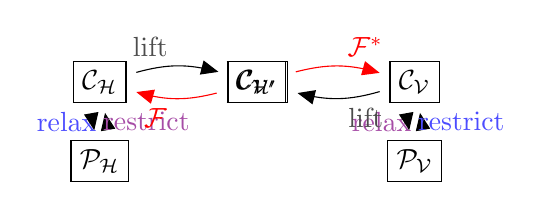
\begin{tikzpicture}[>=triangle 45]
  \node (PH) at (0,0) {\framebox{$\PH$}};
  \node (CH) at (0,\dpos) {\framebox{$\CH$}};
  \node (PV) at (4,0) {\framebox{$\PV$}};
  \node (CV) at (4,\dpos) {\framebox{$\CV$}};
  \node (CVp) at (2,\mhpos) {\framebox{$\CVp$}};
  \node (CHp) at (2,\mlpos) {\framebox{$\CHp$}};
  \draw[->,bend right=10] 
      (PH) to
      node[left,color=blue!70]{relax} 
      (CH);
  \draw[->,bend right=10] 
      (CH) to
      node[right,color=violet!70]{restrict} 
      (PH);
  \draw[->, bend right=10]
      (PV) to
      node[left,color=violet!70]{relax} 
      (CV);
  \draw[->,bend right=10]
      (CV) to
      node[right, color=blue!70]{restrict} 
      (PV);
  \draw[->,bend left=15]
      (CH) to
      node[above left,color=black!70]{lift}
      (CVp);
  \draw[->,bend left=15, color=red]
      (CVp) to
      node[above right]{$\F^*$}
      (CV);
  \draw[->,bend left=15]
      (CV) to
      node[below right,color=black!70]{lift}
      (CHp);
  \draw[->,bend left=15,color=red]
      (CHp) to
      node[below left]{$\F$}
      (CH);
\end{tikzpicture}
\caption{Diagram of the proof}
\label{fig:proof}
\end{centering}
\end{figure}


\subsection{Overview}
The proof shall proceed by first considering an H-Polyhedron $\PH$, and constructing from it a V-Polyhedron $\PV$ which represents the same set of points, then starting with a V-Polyhedron $\PV$ and constructing an H-Polyhedron $\PH$.  The high-level steps are almost identical, and is illustrated in Figure \ref{fig:proof}.

First, $\PH$ will be relaxed to a cone $\CH$.  While technically unnecessary, in the steps that follow it is convenient to have a cone, as opposed to a more general polyhedron.  $\CH$ is then immediately lifted to a higher dimension so that it can be directly represented as a V-Cone $\CV$ \todo{have we defined V-Cone?}.  It is at this point that the ``real work'' must be done (which is why this arrow is colored red).  This step requires intersecting the V-Cone with a number of hyperplanes, and requires a process which is dual to the so-called ``\FME.''  At this point, a simple observation will allow us to restrict $\CV$ to get us to $\PV$, completing this direction of the proof.  Note that this restriction is the opposite of the relaxation which occurs at the beginning of this direction of the proof, as the colors of the diagram reflect.

For the other direction, the exact same steps are taken, however the relaxing and lifting that occur are designed to convert the V-Polyhedron into a V-Cone and H-Cone, instead of the other way around$^1$.  Also, the full fledged ``\FME'' shall take place, this time because we need to project an H-Cone down a number of dimensions.

The transformation which go from $V \to H$ and $H \to V$ representations in the proof seem like a bit of trickery, but in earnest these come from the field of Linear Programming.  For more information on these types of transformations, and a more systematic treatment of them, see \todo{that book by Matusek...}, for instance.

\medskip
Finally, before we get started, I'd like to mention that Ziegler provides the questions:
\begin{itemize}
  \item ``Is a polyhedron intersected with a hyperplane also a polyhedron?''
  \item ``Is the projection of a polyhedron also a polyhedron?''
\end{itemize}
as examples of the utility of the two different representations.  The answer to the first question is clear for H-Polyhedra, this is merely adding another constraint to the system, while it is not so clear for a V-Polyhedra (it seems as though you must somehow ``solve'' something to prove this...)  Similarly, the second question is clear for V-Polyhedra, you simply take the vectors that you already have and forget about some of the coordinates, while for H-Polyhedra it again seems like some system needs to somehow be solved in order to prove this statement.  Before you go and try to prove it yourself, know that the ``solving'' of these problems is essentially \FME, and is the bulk of the work in the proof that follows.

\subsection{H-Polyhedra $\to$ V-Polyhedra}
\paragraph{Overview}
As Figure \ref{fig:proof} indicates, the proof in this direction will generally be of the following form:
  \[ \PH \to \CH \to \CVp \to \CV \to \PV \]
It should then be of no surprise that the actual proof is essentially just elucidating this diagram.

\subsubsection{Relax: $\PH \to \CH$} 
This is a straightforward step.  Let $\PH = \{x : A\x \leq \b\}$ for some $A$ and $\b$.  To achieve the form of a cone, the right hand side of the inequality needs to be $0$.  In order to do this, we prepend $\b$ to the matrix $A$, and introduce a new variable as follows:
  \[ A\x \leq \b \to [\b|A] \xx \leq 0 \]
Observe that this is in fact a relaxation to an H-Cone.  The restriction back to the original H-Polyhedron is to intersect the H-Cone with the hyperplane $\{\x : x_0 = 1\}$, that is:
  \[ \PH = \left\{ [\b|A] \xx \leq 0 \right\} \cap \{ \x : x_0 = 1 \} \]
For now, we deal with the relaxed cone $\CH$ and do this restriction as the last step in the proof of this direction.  In what follows, $A' = [\b|A]$ and $\x' = \xx$.  This notation will simplify the expressions that follow.

\subsubsection{Lift: $\CH \to \CVp$}
The task is to \textit{somehow} go from dealing with halfspaces to dealing with rays.  This step is deceptively ``easy,'' in that it requires a good idea.  Let $A^i$ denote the $i$-th column of $A$.  Observe that $A\x = \sum_i A^i\cdot x_i$.  The significance of this is that matrix multiplication can be considered in two fundamentally different ways, as either: a number of dot products $\dotproduct{\a_i}{\x}$, or as a linear combination of column vectors $\sum_i A^i\cdot x_i$.  This important difference is key to representing the inequality above as a cone.  Suppose that $A \in \R^{m\times n}$, i.e. that $A$ as $m$ rows, and consider the vector $x_i\cdot\smallstack{\e_i}{A^i} \in \R^{n + m}$.  Here, the first $n$ rows keep track of the \textit{value} and \textit{position} of the contribution of $x_i$ (a scalar) to the vector $\x$, while the bottom $m$ rows correspond to the contribution of $x_i$ to the \textit{sum} $\sum_i A^i\cdot x_i$.

Let $\pi_{\x} : \R^{n+m} \to \R^{n}$ be a projection to the first $n$ coordinates, and $\pi^{\x} : \R^{n+m} \to \R^{m}$ a projection to the last $m$ coordinates.  Now, consider the sum 
  \[ \sum\nolimits_i x_i \stack{\e_i}{A^i} = \stack{\x}{A\x} \]
This equality follows from the discussion that precedes it, and it is quite significant, mostly because:
  \[ \pi_{\x} \stack{\x}{A\x}\ = \x,\quad \pi^{\x} \stack{\x}{A\x}\ = A\x \]
\todo{I think that switching the notation of ``projection to'' and ``projection from'' would be in order}
Without further adieu, consider the cone:
  \[ \mathcal{C}_0 = \cone\left(\left\{\pm\stack{\e_i}{A^i}\right\}\right) \]
What are the members of this cone?  Say $\smallstack{\x}{\z} \in \mathcal{C}_0$, then this vector must be a positive linear combination of its generators \todo{define generators}.  In other words:
  \[ \exists\, t^+_i, t^-_i \geq 0 \left| \stack{\x}{\z} = 
       \sum\nolimits_i t^+_i \cdot\stack{\e_i}{A^i} + 
                       t^-_i \cdot{-\!\!\stack{\e_i}{A^i}} \right. =
       \sum\nolimits_i (t^+_i - t^-_i) \cdot\stack{\e_i}{A^i}
   \]
Letting $t_i = (t^+_i - t^-_i)$ in the above equations, and noting that $t_i$ can range over all of $\R$, we get:
  \[ \exists t_i \in \R \left| \stack{\x}{\z} = \sum\nolimits_i t_i \cdot\stack{\e_i}{A^i} \right.
       \Rightarrow \z = A\x \]
To recap what has been accomplished, we have created a V-Cone, in which the first $n$ coordinates keep track of some values corresponding to a vector we've been calling $\x$, and the final $m$ coordinates keep track of the result of the multiplication $A\x$.  This V-Cone becomes powerful when we fix $\z$, that is, taking the V-Cone's intersection with a set of the form $\{\smallstack{\x}{\z} \suchthat \z = \b\}$ for some carefully chosen vector $\b$.  Then, we take a projection of this new set formed by intersection, and recover useful values of $\x$, that is:
  \[ \pi_{\x}\left(\mathcal{C}_0 \cap 
             \left\{\stack{\x}{\z} \bigg|\; \z = \b \right\}\right) =
     \left\{\x \suchthat A\x = \b\right\} 
  \]
In this way, we can recover the solutions to the equation $A\x = \b$.  As previously mentioned, the projection of a V-Cone is easy to deal with, just restrict the generators to the desired coordinates, but the intersection is a bit trickier to deal with, and is the subject of the next part of the proof.  There is one more loose end to tie up before we go on.

As of right now, we have an alleged way to get the solutions of $A\x = \b$ from a V-Cone, but what we really need are the solutions to $A\x \leq \b$.  There is a quick and dirty way to get this from $\mathcal{C}_0$, through introducing what are known in linear programming circles as \textit{slack variables.}  This is just a form of relaxation.

Suppose that you have an $\x$ such that $A\x \leq \b$, and let $\w = \b - A\x$.  This $\w$ can be thought of as \textit{slack}, and is the key to getting from $\mathcal{C}_0$ to $\CVp$.  The key property of this slack is $0 \leq \w$, so $\w$ can be written as
  \[ \w = \sum\nolimits_j w_j\cdot\e_j 
          \Rightarrow \exists\,w_j \geq 0 \;\big|\; \w = \sum\nolimits_j w_j\cdot\e_j \]
Now, we add these bases vectors $\e_j$ to the generators of $\mathcal{C}_0$ to create $\CVp$:
  \[ \CVp = \cone\left(\left\{\pm\stack{\e_i}{A^i}\right\} \cup 
                 \left\{\stack{\vec{0}}{\e_j}\right\}\right) 
  \]
As before, we fix the last $m$ coordinates, carefully choosing our $\b$ to be $\vec{0}$, and again projecting to the coordinates that interest us:
  \[ \pi_{\x} \left( \CVp \cap \left\{\stack{\x}{\z} \bigg|\; \z = \vec{0}\right\} \right) = 
               \{\x \suchthat A\x \leq \vec{0}\}
  \]

\subsubsection{Drop: $\CVp \to \CH$}
Now we turn to intersecting $\CVp$ with $\left\{\smallstack{\x}{\z} |\, \z = \vec{0}\right\}$.

\subsection{V-Polyhedra $\to$ H-Polyhedra}
% by arrow


%
%\section{Program}
%
%% overview
%% design principles
%% details
%% correctness
%% complexity
%
%\section{Discussion}
%\input{mwt_discussion}
%% representations / polymorphism
%% algorithms
%% other proofs
%
\end{document}
